\chapter{On-Off Keying (OOK)}
\label{ch:ook}

\begin{nontechnical}
\textbf{OOK is literally just turning a signal ON and OFF}---it's the simplest possible way to send data, like Morse code with a flashlight!

\textbf{Simple idea:}
\begin{itemize}
\item Bit 1 = signal ON (carrier present)
\item Bit 0 = signal OFF (no carrier)
\end{itemize}

\textbf{Real use:} Your car key fob, garage door opener, and wireless doorbell all use OOK. Press the button, it turns the radio signal on and off to send the unlock code.

\textbf{Why so simple?} Ultra-low cost hardware (< \$2 for transmitter + receiver), minimal power consumption (no signal = no power for 0s), and good enough for short-range low-speed links. Trade-off: Poor noise performance, needs 3~dB more power than BPSK.
\end{nontechnical}

\section{Overview}

\textbf{On-Off Keying (OOK)} is the simplest form of digital modulation, where binary data is encoded by the \textbf{presence or absence} of a carrier wave.

\begin{keyconcept}
OOK is a special case of Amplitude-Shift Keying (ASK) where one amplitude level is \textbf{zero}. This makes it the easiest modulation to implement in hardware---a single transistor switch can serve as a complete transmitter.
\end{keyconcept}

OOK was the first modulation scheme ever used in wireless communications (Marconi's telegraph, 1895) and remains ubiquitous in cost-sensitive, short-range applications such as RFID tags, key fobs, and wireless sensors.

\section{Mathematical Description}

\subsection{Time-Domain Signal}

The OOK waveform is expressed as:
\begin{equation}
s(t) = b_k \cdot A \cos(2\pi f_c t) \quad \text{for} \quad kT_b \leq t < (k+1)T_b
\end{equation}
where:
\begin{itemize}
\item $A$ = carrier amplitude (volts)
\item $f_c$ = carrier frequency (Hz)
\item $T_b$ = bit duration (seconds)
\item $b_k \in \{0, 1\}$ = data bit
\end{itemize}

\textbf{Bit encoding:}
\begin{equation}
s(t) = \begin{cases}
A \cos(2\pi f_c t) & \text{if bit = 1 (carrier ON)} \\
0 & \text{if bit = 0 (carrier OFF)}
\end{cases}
\end{equation}

\begin{calloutbox}{Physical Interpretation}
OOK is effectively \textbf{on-off switching} of a continuous wave carrier. The transmitter literally turns the carrier on and off in sync with the binary data stream. This makes implementation trivial: a single RF switch controlled by the data signal.
\end{calloutbox}

\subsection{Energy and Power}

\textbf{Energy per bit:}
\begin{equation}
E_b = \frac{1}{2} \int_0^{T_b} A^2 \cos^2(2\pi f_c t)\,dt = \frac{A^2 T_b}{4}
\end{equation}

Note: Average energy is $E_b/2$ (assuming equal probability of 0s and 1s), since ``0'' bits transmit no energy.

\textbf{Average transmitted power:}
\begin{equation}
P_{\text{avg}} = \frac{A^2}{4} \cdot P(b_k = 1) = \frac{A^2}{8} \quad \text{(for equiprobable bits)}
\end{equation}

\section{IQ Representation}

The baseband complex representation of OOK is:
\begin{equation}
s(t) = \mathrm{Re}\{b_k \cdot A \cdot e^{j2\pi f_c t}\}
\end{equation}

\textbf{IQ components:}
\begin{itemize}
\item \textbf{I (In-phase):} $I_k = b_k \cdot A$ (either $A$ or $0$)
\item \textbf{Q (Quadrature):} $Q_k = 0$ (OOK uses only the I axis)
\end{itemize}

\subsection{Constellation Diagram}

The OOK constellation consists of two points on the real axis with unequal spacing from the origin:

\begin{center}
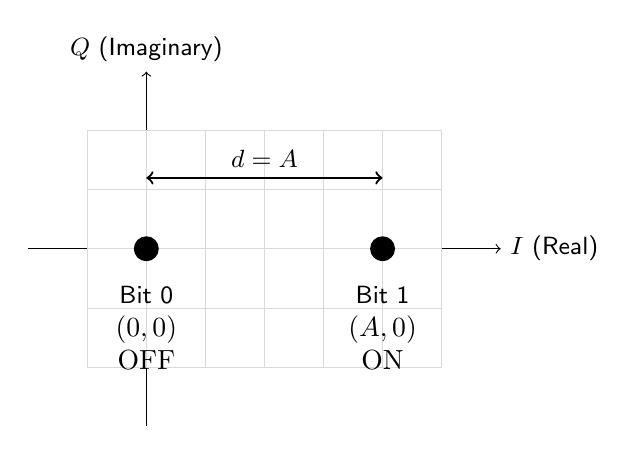
\begin{tikzpicture}[scale=1.5]
% Axes
\draw[->] (-1,0) -- (3,0) node[right] {\sffamily\small $I$ (Real)};
\draw[->] (0,-1.5) -- (0,1.5) node[above] {\sffamily\small $Q$ (Imaginary)};

% Grid
\draw[very thin,gray!30] (-0.5,-1.0) grid[step=0.5] (2.5,1.0);

% Constellation points
\fill[black] (0,0) circle (3pt);
\fill[black] (2,0) circle (3pt);

% Labels
\node[below=10pt,align=center] at (0,0) {\sffamily\small Bit 0\\$(0, 0)$\\OFF};
\node[below=10pt,align=center] at (2,0) {\sffamily\small Bit 1\\$(A, 0)$\\ON};

% Distance annotation
\draw[<->,thick] (0,0.6) -- (2,0.6) node[midway,above] {\sffamily\small $d = A$};
\end{tikzpicture}
\end{center}

\begin{warningbox}
\textbf{Suboptimal spacing.} Unlike BPSK which uses $\pm A$ (distance $d = 2A$), OOK uses $\{0, A\}$ (distance $d = A$). This \textbf{halves the Euclidean distance} between symbols, resulting in a 3~dB performance penalty for the same average power.
\end{warningbox}

\section{Modulation and Demodulation}

\subsection{Transmitter (Modulator)}

The OOK modulator is the simplest of all digital modulation schemes:

\begin{center}
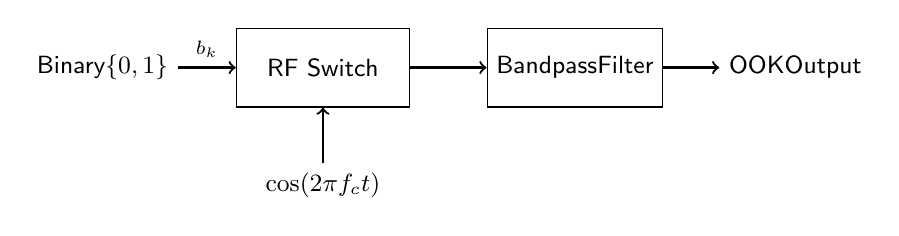
\begin{tikzpicture}[
  block/.style={rectangle, draw, minimum width=2.2cm, minimum height=1cm, font=\sffamily\small},
  node distance=2.2cm,
  font=\small
]
\node (input) {\sffamily Binary\\$\{0, 1\}$};
\node[block, right of=input, node distance=2.8cm] (switch) {RF Switch};
\node[block, right of=switch, node distance=3.2cm] (filter) {Bandpass\\Filter};
\node[right of=filter, node distance=2.8cm] (output) {\sffamily OOK\\Output};

\node[below of=switch, node distance=1.5cm, font=\small] (carrier) {$\cos(2\pi f_c t)$};

\draw[->,thick] (input) -- node[above,font=\scriptsize] {$b_k$} (switch);
\draw[->,thick] (carrier) -- (switch);
\draw[->,thick] (switch) -- (filter);
\draw[->,thick] (filter) -- (output);
\end{tikzpicture}
\end{center}

\textbf{Process:}
\begin{enumerate}
\item \textbf{RF switch:} Data bit controls carrier on/off
  \begin{itemize}
  \item Bit 1 $\rightarrow$ switch closed $\rightarrow$ carrier passes
  \item Bit 0 $\rightarrow$ switch open $\rightarrow$ no output
  \end{itemize}
\item \textbf{Bandpass filter:} Limits spectral occupancy (pulse shaping)
\end{enumerate}

\subsection{Receiver (Non-Coherent Detector)}

OOK is almost always demodulated using \textbf{non-coherent detection} (envelope detection) to avoid the complexity of carrier recovery:

\begin{center}
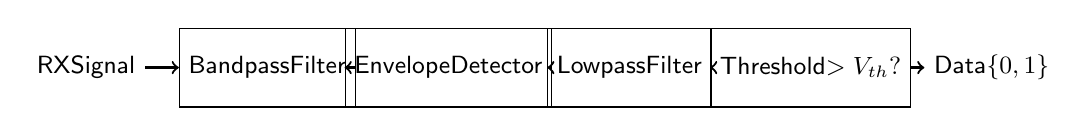
\begin{tikzpicture}[
  block/.style={rectangle, draw, minimum width=1.8cm, minimum height=1cm, font=\sffamily\small},
  node distance=2cm,
  font=\small
]
\node (input) {\sffamily RX\\Signal};
\node[block, right of=input, node distance=2.3cm] (bpf) {Bandpass\\Filter};
\node[block, right of=bpf, node distance=2.3cm] (env) {Envelope\\Detector};
\node[block, right of=env, node distance=2.3cm] (lpf) {Lowpass\\Filter};
\node[block, right of=lpf, node distance=2.3cm] (thresh) {Threshold\\$>V_{th}?$};
\node[right of=thresh, node distance=2.3cm] (output) {\sffamily Data\\$\{0,1\}$};

\draw[->,thick] (input) -- (bpf);
\draw[->,thick] (bpf) -- (env);
\draw[->,thick] (env) -- (lpf);
\draw[->,thick] (lpf) -- (thresh);
\draw[->,thick] (thresh) -- (output);
\end{tikzpicture}
\end{center}

\textbf{Detection process:}

\begin{enumerate}
\item \textbf{Bandpass filter:} Select desired signal, reject out-of-band noise

\item \textbf{Envelope detector:} Rectify and extract amplitude
\begin{equation}
e(t) = |r(t)| = \sqrt{I^2(t) + Q^2(t)}
\end{equation}

\item \textbf{Lowpass filter:} Smooth envelope, remove carrier remnants

\item \textbf{Threshold decision:}
\begin{equation}
\hat{b}_k = \begin{cases}
1 & \text{if } e(t) > V_{th} \quad \text{(carrier detected)} \\
0 & \text{if } e(t) < V_{th} \quad \text{(no carrier)}
\end{cases}
\end{equation}
\end{enumerate}

\textbf{Optimal threshold:} For equiprobable bits in AWGN:
\begin{equation}
V_{th} = \frac{A}{2}
\end{equation}

\begin{keyconcept}
\textbf{No carrier recovery needed!} Envelope detection works without knowing the carrier phase, making OOK the simplest modulation to demodulate. A basic hardware implementation uses just a diode, capacitor, and comparator.
\end{keyconcept}

\section{Bit Error Rate (BER) Performance}

\subsection{Non-Coherent OOK in AWGN Channel}

For envelope detection with optimal threshold:
\begin{equation}
\mathrm{BER} = \frac{1}{2}e^{-E_b/(2N_0)}
\end{equation}
where:
\begin{itemize}
\item $E_b = \frac{A^2 T_b}{4}$ = energy per bit (joules)
\item $N_0$ = noise power spectral density (W/Hz)
\end{itemize}

\textbf{Performance benchmarks:}

\begin{center}
\begin{tabular}{@{}lrl@{}}
\toprule
$E_b/N_0$ (dB) & \multicolumn{1}{c}{BER} & Practical Meaning \\
\midrule
0~dB & $3.0 \times 10^{-1}$ & 3 errors in 10 bits \\
5~dB & $8.2 \times 10^{-2}$ & 1 error in 12 bits \\
10~dB & $6.7 \times 10^{-3}$ & 1 error in 150 bits \\
15~dB & $5.5 \times 10^{-4}$ & 1 error in 1,800 bits \\
\bottomrule
\end{tabular}
\end{center}

\subsection{Coherent OOK (Rarely Used)}

If carrier recovery is available (defeating the main advantage of OOK):
\begin{equation}
\mathrm{BER} = Q\left(\sqrt{\frac{E_b}{N_0}}\right) = \frac{1}{2}\mathrm{erfc}\left(\sqrt{\frac{E_b}{2N_0}}\right)
\end{equation}

Coherent detection provides approximately 1~dB improvement over non-coherent, but is rarely implemented in OOK systems due to added complexity.

\subsection{Comparison: OOK vs BPSK}

At the same average transmitted power:

\begin{center}
\begin{tabular}{@{}lrr@{}}
\toprule
Modulation Scheme & $E_b/N_0$ for $10^{-6}$ BER & Performance \\
\midrule
OOK (non-coherent) & 13.5~dB & Baseline \\
\textbf{BPSK (coherent)} & \textbf{10.5~dB} & \textbf{3~dB better} \\
\bottomrule
\end{tabular}
\end{center}

\begin{keyconcept}
\textbf{Why is BPSK 3~dB better than OOK?}

\begin{enumerate}
\item \textbf{Distance between constellation points:} BPSK uses $\{-A, +A\}$ (separation $2A$), while OOK uses $\{0, A\}$ (separation $A$). Doubling the distance quadruples noise immunity.

\item \textbf{Energy utilization:} BPSK transmits energy continuously. OOK transmits only during ``1'' bits, wasting half the signal space.

\item \textbf{Coherent vs non-coherent:} Coherent detection (BPSK) is optimal. Non-coherent detection (OOK) loses 1~dB additionally.
\end{enumerate}
\end{keyconcept}

\section{Bandwidth Efficiency}

The occupied bandwidth (99\% power) for rectangular pulses is:
\begin{equation}
B \approx \frac{2}{T_b} = 2R_b
\end{equation}
where $R_b$ is the bit rate (bps) and $T_b$ is the bit period (seconds).

OOK requires \textbf{twice the bandwidth of BPSK} for the same data rate due to the on-off transitions creating spectral spreading.

With \textbf{pulse shaping} (raised-cosine filter, roll-off factor $\alpha$):
\begin{equation}
B = 2R_b(1 + \alpha)
\end{equation}

\textbf{Spectral efficiency:}
\begin{equation}
\eta = \frac{R_b}{B} = \frac{1}{2(1+\alpha)} \approx 0.37\ \text{bps/Hz} \quad \text{(for $\alpha = 0.35$)}
\end{equation}

This is \textbf{half the spectral efficiency of BPSK} ($\sim$0.74~bps/Hz).

\section{Practical Implementations}

\subsection{Passive RFID Tags (EPC Gen2)}

The primary modern application of OOK is in \textbf{passive RFID} (Radio-Frequency Identification):

\begin{itemize}
\item \textbf{Frequency:} 860--960~MHz (UHF band)
\item \textbf{Modulation:} OOK or ASK for tag-to-reader uplink (backscatter)
\item \textbf{Data rate:} 40--640~kbps
\item \textbf{Range:} 1--10~m (depending on reader power and tag antenna)
\item \textbf{Power:} Tag harvests energy from reader's carrier wave
\end{itemize}

\textbf{Backscatter mechanism:}
\begin{enumerate}
\item Reader transmits continuous wave (CW) carrier
\item Tag modulates its antenna impedance (switch between matched/mismatched)
\item Matched load $\rightarrow$ absorbs power (bit 0)
\item Mismatched load $\rightarrow$ reflects power (bit 1)
\item Reader detects reflected signal modulation
\end{enumerate}

\begin{calloutbox}[colback=black!5!white,colframe=black]{Example: Walmart RFID Inventory System}
\begin{tabular}{@{}ll@{}}
Application & Retail inventory tracking \\
Frequency & 902--928~MHz (FCC Part 15) \\
Reader TX power & 1~W EIRP (30~dBm) \\
Tag sensitivity & $-18$~dBm \\
Read range & 5--7~m \\
Throughput & 1,000 tags/second \\
Cost per tag & \$0.05--\$0.15 (bulk) \\
\end{tabular}

\vspace{0.3cm}
\textbf{Why OOK?} Ultra-low complexity allows battery-free operation. The tag IC draws < 20~$\mu$W from the harvested RF field.
\end{calloutbox}

\subsection{Wireless Key Fobs and Remote Controls}

Consumer electronics use OOK at 315~MHz (USA) or 433~MHz (Europe/Asia):

\begin{itemize}
\item \textbf{Car key fobs:} Unlock/lock commands (< 1~kbps)
\item \textbf{Garage door openers:} Fixed or rolling codes
\item \textbf{Wireless doorbells:} Simple on-off signaling
\item \textbf{Tire pressure monitors:} Low-duty-cycle sensor data
\end{itemize}

\textbf{Typical specifications:}
\begin{itemize}
\item TX power: 1--10~mW
\item Data rate: 1--10~kbps
\item Range: 10--100~m (line of sight)
\item Modulation: OOK with Manchester or PWM encoding
\end{itemize}

\subsection{Optical Communications}

In fiber optics, OOK (called ``intensity modulation'') is ubiquitous:

\begin{itemize}
\item \textbf{10 Gigabit Ethernet:} 10.3125~Gbps OOK with direct detection
\item \textbf{PON (Passive Optical Networks):} 1--10~Gbps OOK for residential fiber
\item \textbf{Free-space optical:} LED/laser on-off for visible light communication (VLC)
\end{itemize}

\textbf{Advantages in optical domain:}
\begin{itemize}
\item Laser diodes are inherently on-off devices
\item Photodetectors naturally perform envelope detection
\item No need for phase recovery (incoherent detection)
\item Simpler than coherent optical modulation (QPSK, QAM)
\end{itemize}

\section{Advantages and Disadvantages}

\subsection*{Advantages}

\begin{enumerate}
\item \textbf{Simplest implementation:} Single RF switch serves as complete modulator
\item \textbf{No carrier recovery:} Envelope detection eliminates synchronization complexity
\item \textbf{Low-power ``0'' bits:} Ideal for low duty-cycle applications (transmit only when needed)
\item \textbf{Ultra-low cost:} < \$0.50 for complete transmitter in bulk (transistor + crystal)
\item \textbf{Battery-free operation:} Enables passive RFID and energy-harvesting sensors
\end{enumerate}

\subsection*{Disadvantages}

\begin{enumerate}
\item \textbf{Poor power efficiency:} 3~dB penalty versus BPSK for same BER
\item \textbf{Poor spectral efficiency:} $\sim$0.37~bps/Hz (half of BPSK)
\item \textbf{Threshold sensitivity:} Performance degrades if decision threshold is not optimal
\item \textbf{Susceptible to fading:} Deep fades eliminate the carrier entirely (no diversity)
\item \textbf{DC wander:} Long sequences of 0s or 1s cause baseline drift in envelope detector
\end{enumerate}

\section{Worked Example: Passive RFID Link Budget}

\textbf{Scenario:} UHF RFID reader interrogating a passive tag at 915~MHz

\subsection*{Given Parameters}

\begin{tabular}{@{}ll@{}}
Reader TX power & $P_t = 1$~W = 30~dBm (FCC limit) \\
Reader antenna gain & $G_t = 6$~dBi (circularly polarized) \\
Tag antenna gain & $G_{tag} = 2$~dBi (dipole) \\
Distance & $d = 5$~m \\
Frequency & $f = 915$~MHz \\
Tag sensitivity & $P_{tag} = -18$~dBm (power needed to activate) \\
Backscatter modulation & $m = 0.5$ (50\% depth) \\
Reader RX sensitivity & $P_{rx,min} = -70$~dBm \\
\end{tabular}

\subsection*{Step 1: Forward Link (Reader $\rightarrow$ Tag)}

Free-space path loss at 915~MHz:
\begin{equation}
\mathrm{FSPL\,[dB]} = 20\log_{10}(d_m) + 20\log_{10}(f_{\text{MHz}}) + 32.45
\end{equation}
\begin{equation}
\mathrm{FSPL} = 20\log_{10}(5) + 20\log_{10}(915) + 32.45 = 91.2~\text{dB}
\end{equation}

Power received by tag:
\begin{equation}
P_{tag} = P_t + G_t + G_{tag} - \mathrm{FSPL}
\end{equation}
\begin{equation}
P_{tag} = 30 + 6 + 2 - 91.2 = -53.2~\text{dBm}
\end{equation}

\subsection*{Step 2: Forward Link Margin}

\begin{itemize}
\item \textbf{Required power:} $-18$~dBm (tag activation threshold)
\item \textbf{Available power:} $-53.2$~dBm
\item \textbf{Link margin:} $-53.2 - (-18) = -35.2$~dB \textbf{(FAILS!)}
\end{itemize}

\begin{calloutbox}[colback=red!10!white,colframe=red]{Forward Link is Power-Limited}
At 5~m, the tag receives only $-53.2$~dBm, far below the $-18$~dBm needed to power up. Maximum read range is approximately:

\begin{equation}
d_{max} = 5 \times 10^{35.2/20} \approx 0.9~\text{m}
\end{equation}

This illustrates why passive RFID is inherently short-range: the tag must harvest enough power from the RF field to operate its circuitry before it can backscatter a response.
\end{calloutbox}

\subsection*{Step 3: Reverse Link (Tag $\rightarrow$ Reader)}

Assuming the tag is activated (at $d < 1$~m), backscattered power:
\begin{equation}
P_{backscatter} = P_{tag} + \mathrm{backscatter\_gain} - \mathrm{FSPL}
\end{equation}

For OOK backscatter with 50\% modulation depth:
\begin{equation}
P_{rx} = P_t + 2G_t + 2G_{tag} - 2 \times \mathrm{FSPL} - L_{backscatter}
\end{equation}

\textbf{Backscatter loss} $L_{backscatter} \approx 10$~dB (antenna mismatch modulation).

At $d = 0.9$~m:
\begin{equation}
P_{rx} = 30 + 12 + 4 - 2(81.3) - 10 = -126.6~\text{dBm}
\end{equation}

\begin{itemize}
\item \textbf{Reader sensitivity:} $-70$~dBm
\item \textbf{Received backscatter:} $-126.6$~dBm \textbf{(FAILS!)}
\end{itemize}

\textbf{Conclusion:} Passive RFID operates in a power-limited regime where forward link (tag activation) dominates the link budget. Commercial systems use higher reader power (permitted under FCC Part 15.247), better antennas ($G_t > 10$~dBi), and optimized tag ICs to achieve 5--10~m ranges.

\section{Relationship to Other Modulations}

\subsection{Amplitude-Shift Keying (ASK)}

OOK is a special case of \textbf{M-ary ASK} with $M = 2$ and one amplitude level at zero:
\begin{equation}
s(t) = A_k \cos(2\pi f_c t) \quad \text{where} \quad A_k \in \{0, A\}
\end{equation}

General ASK uses non-zero levels: $A_k \in \{A_1, A_2, \ldots, A_M\}$ where $A_1 > 0$.

\textbf{Advantage of non-zero levels:} Reduces DC wander and improves timing recovery, but increases average power.

\textbf{Visual comparison:} OOK extends naturally to higher-order ASK by adding amplitude levels:

\begin{center}
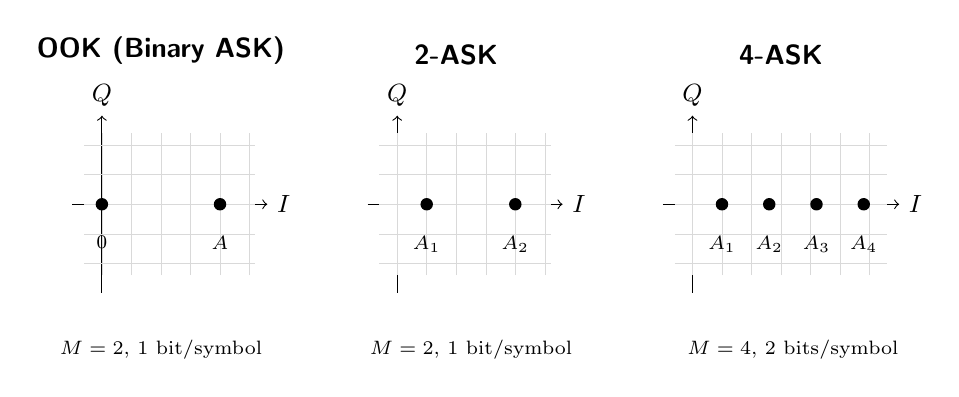
\begin{tikzpicture}[scale=0.75]
% OOK (Binary ASK)
\begin{scope}[shift={(0,0)}]
\node[above,font=\sffamily\bfseries] at (1,2.2) {OOK (Binary ASK)};
\draw[->] (-0.5,0) -- (2.8,0) node[right,font=\sffamily\small] {$I$};
\draw[->] (0,-1.5) -- (0,1.5) node[above,font=\sffamily\small] {$Q$};
\draw[very thin,gray!30] (-0.3,-1.2) grid[step=0.5] (2.6,1.2);
\fill[black] (0,0) circle (3pt);
\fill[black] (2,0) circle (3pt);
\node[below=8pt,font=\scriptsize] at (0,0) {0};
\node[below=8pt,font=\scriptsize] at (2,0) {$A$};
\node[below=20pt,font=\scriptsize] at (1,-1.2) {$M=2$, 1 bit/symbol};
\end{scope}

% 2-ASK (Non-zero levels)
\begin{scope}[shift={(5,0)}]
\node[above,font=\sffamily\bfseries] at (1,2.2) {2-ASK};
\draw[->] (-0.5,0) -- (2.8,0) node[right,font=\sffamily\small] {$I$};
\draw[->] (0,-1.5) -- (0,1.5) node[above,font=\sffamily\small] {$Q$};
\draw[very thin,gray!30] (-0.3,-1.2) grid[step=0.5] (2.6,1.2);
\fill[black] (0.5,0) circle (3pt);
\fill[black] (2,0) circle (3pt);
\node[below=8pt,font=\scriptsize] at (0.5,0) {$A_1$};
\node[below=8pt,font=\scriptsize] at (2,0) {$A_2$};
\node[below=20pt,font=\scriptsize] at (1.25,-1.2) {$M=2$, 1 bit/symbol};
\end{scope}

% 4-ASK
\begin{scope}[shift={(10,0)}]
\node[above,font=\sffamily\bfseries] at (1.5,2.2) {4-ASK};
\draw[->] (-0.5,0) -- (3.5,0) node[right,font=\sffamily\small] {$I$};
\draw[->] (0,-1.5) -- (0,1.5) node[above,font=\sffamily\small] {$Q$};
\draw[very thin,gray!30] (-0.3,-1.2) grid[step=0.5] (3.3,1.2);
\fill[black] (0.5,0) circle (3pt);
\fill[black] (1.3,0) circle (3pt);
\fill[black] (2.1,0) circle (3pt);
\fill[black] (2.9,0) circle (3pt);
\node[below=8pt,font=\scriptsize] at (0.5,0) {$A_1$};
\node[below=8pt,font=\scriptsize] at (1.3,0) {$A_2$};
\node[below=8pt,font=\scriptsize] at (2.1,0) {$A_3$};
\node[below=8pt,font=\scriptsize] at (2.9,0) {$A_4$};
\node[below=20pt,font=\scriptsize] at (1.7,-1.2) {$M=4$, 2 bits/symbol};
\end{scope}
\end{tikzpicture}
\end{center}

\textbf{Key observation:} All ASK modulations use only the I-axis. Unlike PSK (which varies phase) or QAM (which varies both amplitude and phase), ASK is inherently one-dimensional.

\subsection{Comparison Table}

\begin{center}
\begin{tabularx}{\textwidth}{@{}lcXXl@{}}
\toprule
\textbf{Modulation} & \textbf{Bits/Symbol} & \textbf{Bandwidth} & \textbf{$E_b/N_0$ @ BER $10^{-6}$} & \textbf{Complexity} \\
\midrule
\textbf{OOK} & 1 & $2R_b$ & 13.5~dB & Lowest \\
BPSK & 1 & $R_b$ & 10.5~dB & Low \\
QPSK & 2 & $R_b$ & 10.5~dB & Moderate \\
16-QAM & 4 & $R_b$ & 18.5~dB & High \\
\bottomrule
\end{tabularx}
\end{center}

\textbf{Key insight:} OOK trades performance for simplicity. BPSK achieves 3~dB better power efficiency and 2$\times$ better spectral efficiency with only modest increase in complexity.

\section{Summary}

\begin{center}
\begin{tabular}{@{}ll@{}}
\toprule
\textbf{Parameter} & \textbf{Value} \\
\midrule
Bits per symbol & 1 \\
Constellation points & 2 (at $0$ and $A$) \\
Spectral efficiency & $\sim$0.37~bps/Hz (with pulse shaping) \\
BER @ 10~dB $E_b/N_0$ & $6.7 \times 10^{-3}$ (non-coherent) \\
Carrier recovery & Not required (envelope detection) \\
Implementation & Simplest of all modulations \\
Best application & Cost-sensitive, short-range links \\
Typical uses & RFID, key fobs, optical fiber \\
\bottomrule
\end{tabular}
\end{center}

\vspace{0.5cm}

\textbf{Key takeaways:}
\begin{itemize}
\item OOK is the \textbf{simplest digital modulation}---just on/off switching
\item \textbf{No carrier synchronization} required (envelope detection)
\item \textbf{3~dB penalty} versus BPSK due to suboptimal constellation
\item Dominates \textbf{ultra-low-cost} applications (RFID, remotes)
\item Foundation for understanding ASK and other amplitude modulations
\end{itemize}

\section{Further Reading}

\begin{itemize}
\item \textbf{Chapter 4:} Binary Phase-Shift Keying (BPSK)---superior binary alternative
\item \textbf{Chapter 5:} Amplitude-Shift Keying (ASK)---M-ary generalization of OOK
\item \textbf{Chapter 6:} Frequency-Shift Keying (FSK)---alternative simple modulation
\item \textbf{Chapter 7:} Quadrature Phase-Shift Keying (QPSK)---higher spectral efficiency
\item \textbf{Chapter 12:} Constellation Diagrams---visualization techniques
\item \textbf{Chapter 13:} IQ Representation---complex baseband mathematics
\item \textbf{Chapter 18:} Bit Error Rate Analysis---performance measurement
\item \textbf{Chapter 20:} Envelope Detection---non-coherent receiver design
\item \textbf{Chapter 28:} RFID Systems---detailed backscatter link analysis
\end{itemize}
